%% AOA Project 1 — Greedy + Divide-and-Conquer
%% Overleaf: ACM Conference Proceedings (acmart).
\documentclass[sigconf,review=false]{acmart}

%% acmart already loads amsmath, booktabs, graphicx, hyperref, xcolor, etc.
\usepackage{amsthm}
\usepackage{algorithm}
\usepackage{algpseudocode}
\usepackage{listings}
\usepackage{booktabs}

\lstset{
  basicstyle=\ttfamily\footnotesize,
  breaklines=true,
  frame=single,
  numbers=left,
  numberstyle=\tiny,
  keywordstyle=\color{blue!60!black},
  commentstyle=\color{green!40!black},
  language=Python
}

\newtheorem{theorem}{Theorem}
\newtheorem{lemma}[theorem]{Lemma}
\newtheorem{claim}[theorem]{Claim}
\theoremstyle{definition}
\newtheorem{definition}[theorem]{Definition}
\newtheorem{problem}[theorem]{Problem}

\title{Decision-Grade Scheduling and Geospatial Proximity:
Optimal Greedy and Divide-and-Conquer Primitives for
Healthcare Operations and Sensing Networks}

\author{Umesh Chandra Lavu}
\affiliation{%
  \institution{University of Florida}
  \department{Department of Computer \& Information Science \& Engineering}
  \city{Gainesville}
  \state{FL}
  \country{USA}
}
\renewcommand{\shortauthors}{Lavu}

\begin{CCSXML}
<ccs2012>
 <concept>
  <concept_id>10003752.10003809.10003635</concept_id>
  <concept_desc>Theory of computation~Design and analysis of algorithms</concept_desc>
  <concept_significance>500</concept_significance>
 </concept>
 <concept>
  <concept_id>10002950.10003648.10003688</concept_id>
  <concept_desc>Mathematics of computing~Combinatorial optimization</concept_desc>
  <concept_significance>300</concept_significance>
 </concept>
 <concept>
  <concept_id>10010147.10010341</concept_id>
  <concept_desc>Computing methodologies~Computational geometry</concept_desc>
  <concept_significance>300</concept_significance>
 </concept>
</ccs2012>
\end{CCSXML}

\ccsdesc[500]{Theory of computation~Design and analysis of algorithms}
\ccsdesc[300]{Mathematics of computing~Combinatorial optimization}
\ccsdesc[300]{Computing methodologies~Computational geometry}

\begin{document}

\begin{abstract}
Modern enterprises continuously convert messy operational requests into
high-stakes decisions: which patient cases a scarce procedure room can
complete today, and which sensing assets are dangerously close for
quality control or consolidation. We formalize two such decisions as
combinatorial primitives with \emph{exact} optimality guarantees.
First, single-resource appointment selection is modeled as
maximum-cardinality interval scheduling and solved by an
earliest-finish-time greedy algorithm. Second, nearest-asset discovery
in a regional weather (or logistics) network is modeled as closest pair
of points and solved by a divide-and-conquer procedure. For each problem
we supply a set-theoretic abstraction, production-ready pseudocode,
asymptotic analysis, a correctness proof, an operations-facing
explanation, and experimental evidence that observed runtimes track the
predicted $O(n\log n)$ envelope---the performance class expected of
online decision services rather than overnight batch jobs.
\end{abstract}

\keywords{operations research, greedy algorithms, divide and conquer,
interval scheduling, closest pair, healthcare capacity, geospatial
analytics, experimental algorithmics}

\maketitle

%% ------------------------------------------------------------------
\section{Introduction}
\label{sec:intro}
%% ------------------------------------------------------------------

In competitive service organizations, algorithm quality is not an academic
curiosity: it determines throughput, risk exposure, and whether analysts
can act inside an operational time window. Two recurring patterns appear
across healthcare systems and large-scale sensing infrastructures.

\paragraph{Scarce capacity allocation.}
Ambulatory surgical and specialty clinics routinely dedicate a single
procedure room to a time block. Overnight demand often exceeds capacity,
so coordinators must accept a conflict-free subset of requests that
maximizes completed cases~\cite{gupta2015or,cayirli2003}. Heuristics that
``feel fair'' can silently discard capacity; an optimal combinatorial
policy is preferable when the objective is clear.

\paragraph{Asset proximity intelligence.}
National and regional observation networks, and analogous private
telematics fleets, maintain thousands of geo-located
instruments~\cite{noaa2020}. Exact nearest-pair queries surface duplicate
coverage, correlated measurement bias, and consolidation candidates.
Approximate clustering can be useful for dashboards, but field decisions
require an exact answer with predictable latency as networks
scale~\cite{deberg2008,cardenas2013}.

This report shows that both problems admit clean abstractions and
\emph{optimal} $O(n\log n)$ algorithms---earliest-finish-time greedy
selection for interval scheduling, and Shamos--Hoey divide-and-conquer for
closest pair~\cite{kt2005,clrs2009,shamos1975}. The contribution is not a
new theorem, but a decision-engineering package: domain framing that
operations leaders recognize, abstractions engineers can implement,
proofs that withstand review, and empirical scaling curves that
procurement and SRE teams can trust.

Sections~\ref{sec:greedy} and~\ref{sec:dac} develop each problem end to
end. Section~\ref{sec:transfer} maps the same primitives to adjacent
enterprise use cases. Section~\ref{sec:exp} reports experimental
validation. Appendices contain validation code and the required
large-language-model usage log.

%% ------------------------------------------------------------------
\section{Greedy: Maximizing Throughput in a Single OR Block}
\label{sec:greedy}
%% ------------------------------------------------------------------

\subsection{Problem identification}
\label{sec:greedy-id}

Consider an outpatient endoscopy suite that owns one procedure room for a
morning block. By 06:00 the board holds $n$ case requests (screening
colonoscopies, diagnostic EGDs, biopsies). Case~$i$ occupies the room from
start time $s_i$ to finish time $f_i$ inclusive of turnover, with
$s_i < f_i$. Two cases conflict if their occupancy intervals overlap. The
operational objective for this study is throughput: accept a largest
possible conflict-free set so the maximum number of patients complete care
in-block. Priority or revenue weighting can be layered later; cardinality
is the right first-principles objective when access equity is the
mandate~\cite{gupta2015or,cayirli2003}. The problem originates in clinic
operations, not in an algorithms textbook.

\subsection{Abstraction}
\label{sec:greedy-abs}

\begin{definition}[Interval instance]
Let $I = \{I_1,\ldots,I_n\}$ be a finite set of half-open intervals
$I_i = [s_i,f_i)$ on the real line, with $s_i < f_i$.
Two intervals $I_i$ and $I_j$ are \emph{compatible} if
$[s_i,f_i) \cap [s_j,f_j) = \emptyset$.
\end{definition}

\begin{problem}[Maximum-cardinality interval scheduling]
Given $I$, compute a compatible subset $S\subseteq I$ of maximum cardinality.
\end{problem}

Half-open intervals encode the enterprise rule that one case may hand off
to the next at an exact timestamp once turnover is folded into $f_i$.

\subsection{Algorithm}
\label{sec:greedy-alg}

The earliest-finish-time (EFT) greedy algorithm sorts requests by finish
time and repeatedly accepts the next request that starts after the room
is free~\cite{kt2005}.

\begin{algorithm}[t]
\caption{Earliest-Finish-Time Interval Scheduling}
\label{alg:eft}
\begin{algorithmic}[1]
\Require Set $I$ of intervals $[s_i,f_i)$
\Ensure Compatible $S\subseteq I$ of maximum cardinality
\State Sort $I$ so that $f_1 \le f_2 \le \cdots \le f_n$
\State $S \gets \emptyset$;\; $t \gets -\infty$
\For{$i = 1$ to $n$}
  \If{$s_i \ge t$}
    \State $S \gets S \cup \{I_i\}$
    \State $t \gets f_i$
  \EndIf
\EndFor
\State \Return $S$
\end{algorithmic}
\end{algorithm}

\subsection{Running-time analysis}
\label{sec:greedy-rt}

Sorting dominates: $O(n\log n)$ comparisons. The linear scan performs
$O(1)$ work per request. Total time is therefore $O(n\log n)$, which is
acceptable for nightly board builds and for interactive what-if tools on
boards with tens of thousands of candidate slots.

\subsection{Proof of correctness}
\label{sec:greedy-proof}

\begin{theorem}
\label{thm:eft}
Algorithm~\ref{alg:eft} returns a compatible set of maximum cardinality.
\end{theorem}

\begin{proof}
Compatibility is immediate: an interval is added only when
$s_i \ge t$, and $t$ is always the finish time of the most recently
accepted interval.

For optimality we use an exchange (``staying ahead'') argument~\cite{kt2005}.
Let $G = \{g_1,\ldots,g_k\}$ be the intervals chosen by EFT, indexed in the
order they were selected, and let $O = \{o_1,\ldots,o_m\}$ be any optimal
compatible set, indexed by increasing finish time. We claim that for every
$r\le k$,
\[
  f(g_r) \le f(o_r),
\]
where $f(\cdot)$ denotes finish time. The claim is proved by induction on
$r$.

For $r=1$, EFT selects a globally earliest-finishing interval, so
$f(g_1)\le f(o_1)$. Assume the claim holds for $r-1$. Because
$f(g_{r-1})\le f(o_{r-1})$ and $O$ is compatible,
$s(o_r)\ge f(o_{r-1})\ge f(g_{r-1})$. Thus $o_r$ is a feasible candidate at
the moment EFT considers intervals after $g_{r-1}$. EFT therefore chooses
$g_r$ with finish time no larger than that of any remaining feasible
interval, in particular $f(g_r)\le f(o_r)$.

Finally, $k\ge m$. Indeed, if $k<m$ then $o_{k+1}$ would be compatible with
$g_k$ because $s(o_{k+1})\ge f(o_k)\ge f(g_k)$, contradicting termination of
EFT. Hence $|G|=|O|$.
\end{proof}

\subsection{Explanation in the problem domain}
\label{sec:greedy-domain}

From a charge-nurse perspective: sort the overnight request list by when
each case would \emph{release} the room, earliest release first. Accept
the first case. Cross off every later request that would still need the
room during that occupancy. Accept the next remaining request that starts
after release, and repeat. Preferring early release is not a fairness
gimmick---it is the unique simple rule that keeps the room available as
soon as possible and therefore maximizes completed patients.

%% ------------------------------------------------------------------
\section{Divide and Conquer: Exact Nearest-Asset Discovery}
\label{sec:dac}
%% ------------------------------------------------------------------

\subsection{Problem identification}
\label{sec:dac-id}

A meteorological agency (or a private agritech / logistics sensing fleet)
operates $n$ fixed instruments with surveyed latitude/longitude. For
redundancy audits, anomaly triage, and capital planning, analysts must
identify the geographically closest pair~\cite{noaa2020}. Extremely close
pairs suggest duplicate reporting, shared microclimate bias, or sites that
can be consolidated. Coordinates are projected to a local planar frame so
Euclidean distance matches ground distance. Approximate methods are
insufficient when the answer triggers a truck roll; the query must remain
\emph{exact} and sub-quadratic as fleets grow into the tens of
thousands~\cite{deberg2008}.

\subsection{Abstraction}
\label{sec:dac-abs}

\begin{definition}[Point set]
Let $P=\{p_1,\ldots,p_n\}\subset\mathbb{R}^2$ with $n\ge 2$, and let
$d(p,q)=\sqrt{(x_p-x_q)^2+(y_p-y_q)^2}$ be Euclidean distance.
\end{definition}

\begin{problem}[Closest pair]
Compute a pair $\{p^*,q^*\}\subseteq P$ minimizing $d(p^*,q^*)$
(ties broken arbitrarily).
\end{problem}

\subsection{Algorithm}
\label{sec:dac-alg}

We use the classical Shamos--Hoey divide-and-conquer
algorithm~\cite{shamos1975,preparata1985,clrs2009,deberg2008}. Points are
pre-sorted by $x$-coordinate. Each recursive call receives an $x$-sorted
array $P_x$ and a $y$-sorted array $P_y$ of the same point set.

\begin{algorithm}[t]
\caption{Closest Pair (divide and conquer)}
\label{alg:cp}
\begin{algorithmic}[1]
\Require $x$-sorted $P_x$, $y$-sorted $P_y$, $|P_x|=n\ge 2$
\Ensure Distance $\delta$ and a realizing pair
\If{$n \le 3$}
  \State \Return brute-force closest pair among $P_x$
\EndIf
\State Let $Q_x$ (resp.\ $R_x$) be the left (resp.\ right) $\lfloor n/2\rfloor$
      (resp.\ $\lceil n/2\rceil$) points of $P_x$; let $L$ be the median $x$
\State Split $P_y$ into $Q_y$ and $R_y$ accordingly
\State $(\delta_L,\cdot) \gets \mathrm{ClosestPair}(Q_x,Q_y)$
\State $(\delta_R,\cdot) \gets \mathrm{ClosestPair}(R_x,R_y)$
\State $\delta \gets \min(\delta_L,\delta_R)$; record the corresponding pair
\State Let strip $S$ be points of $P_y$ with $|x-L|<\delta$, still $y$-sorted
\For{each point $p\in S$ in order}
  \State Compare $p$ to the next points of $S$ whose $y$-gap is $<\delta$
        (at most $7$ successors suffice)
  \State Update $\delta$ and the best pair if a closer pair is found
\EndFor
\State \Return $\delta$ and its pair
\end{algorithmic}
\end{algorithm}

A one-time $O(n\log n)$ sort by $x$ and by $y$ precedes the recursion; each
recursive level rebuilds left/right $y$-lists in linear time.

\subsection{Running-time analysis}
\label{sec:dac-rt}

Let $T(n)$ be the time of the recursive procedure on $n$ points (after the
initial sorts). The base case $n\le 3$ is $O(1)$. Otherwise two subproblems
of size $\lfloor n/2\rfloor$ and $\lceil n/2\rceil$ are solved, and the
combine step (building the strip and scanning $O(1)$ neighbors per strip
point) costs $O(n)$. Therefore
\[
  T(n) = T\!\left(\Big\lfloor\frac{n}{2}\Big\rfloor\right)
       + T\!\left(\Big\lceil\frac{n}{2}\Big\rceil\right) + O(n).
\]
By the Master Theorem (or a recursion-tree argument), $T(n)=O(n\log n)$.
Including the initial sorts does not change the asymptotic bound, so the
full algorithm runs in $O(n\log n)$ time---fast enough for interactive
geospatial audit tools and for nightly fleet health jobs.

\subsection{Proof of correctness}
\label{sec:dac-proof}

\begin{lemma}[Strip property]
\label{lem:strip}
Let $\delta=\min(\delta_L,\delta_R)$. Any pair closer than $\delta$ must
consist of one point from each half and both points must lie in the vertical
strip of width $2\delta$ centered at the dividing line $L$.
\end{lemma}

\begin{proof}
A pair lying entirely in one half has distance at least $\delta$ by
induction. If a cross pair has either point outside the strip, its
horizontal separation is at least $\delta$, so its Euclidean distance is at
least $\delta$.
\end{proof}

\begin{lemma}[Constant neighbor check]
\label{lem:box}
Order the strip by increasing $y$-coordinate. For any strip point $p$, at
most seven subsequent strip points can lie at distance less than $\delta$
from $p$.
\end{lemma}

\begin{proof}[Proof sketch]
Any two points from the same half are at least $\delta$ apart. Packing
disks of radius $\delta/2$ into the $\delta\times 2\delta$ rectangle above
$p$ shows that at most eight centers fit, one of which is $p$
itself~\cite{clrs2009}. Hence at most seven other candidates need checking;
equivalently, one may stop once the $y$-gap reaches $\delta$.
\end{proof}

\begin{theorem}
Algorithm~\ref{alg:cp} returns a closest pair.
\end{theorem}

\begin{proof}
By induction on $n$. The base case $n\le 3$ is exhaustive. For larger $n$,
the recursive calls correctly compute $\delta_L$ and $\delta_R$.
Lemma~\ref{lem:strip} confines any improving pair to the strip, and
Lemma~\ref{lem:box} ensures the linear scan examines every strip pair that
could improve $\delta$. Therefore the returned distance is globally minimal.
\end{proof}

\subsection{Explanation in the problem domain}
\label{sec:dac-domain}

From an operations-analytics perspective: sort assets west-to-east. Recursively
find the closest pair in the western half and in the eastern half; let
$\delta$ be the better of those two distances. The only remaining threat to
that champion is a pair that straddles the dividing meridian and sits inside
a $2\delta$-wide corridor. Walk corridor assets south-to-north and, for each
asset, check only a constant number of neighbors immediately to the north.
The closest pair found anywhere---inside a half or across the divide---is
the network-wide answer that can be escalated to field teams.

%% ------------------------------------------------------------------
\section{Enterprise Transferability}
\label{sec:transfer}
%% ------------------------------------------------------------------

The same abstractions transfer without changing the algorithms:
\begin{itemize}
  \item \textbf{Interval scheduling:} classroom/lab booking, single-bay EV
        charging, broadcast-slot assignment, and exclusive lock windows in
        change-management calendars.
  \item \textbf{Closest pair:} retail store cannibalization checks, cell-tower
        densification audits, warehouse/robot dock proximity, and fraud rings
        that share near-identical geo-signatures.
\end{itemize}
In each case the business value comes from \emph{exactness plus predictable
latency}: leaders can defend the decision, and platforms can budget compute.

%% ------------------------------------------------------------------
\section{Experimental Validation}
\label{sec:exp}
%% ------------------------------------------------------------------

\subsection{Methodology}
We implemented both algorithms in Python~3 and verified functional
correctness against exhaustive oracles (subset enumeration for interval
scheduling on small $n$; quadratic search for closest pair). Timing used
\texttt{time.perf\_counter} wall-clock measurements on synthetic uniform
random instances, averaged across multiple trials and repeats per size.
This methodology mirrors how platform teams validate that an analytic
service remains inside an SLA envelope as load grows.

\subsection{Results}
For OR scheduling we timed $n\in\{2^{10},\ldots,2^{16}\}$. For closest pair
we timed $n\in\{2^{10},\ldots,2^{15}\}$. Table~\ref{tab:timing} summarizes
mean runtimes. Figures~\ref{fig:greedy-rt}--\ref{fig:closest-ratio} compare
measured time to a scaled $c\,n\log n$ reference and plot the normalized
cost $T(n)/(n\log_2 n)$. Near-constant normalized cost, together with
alignment on log--log axes, empirically supports the $O(n\log n)$ analyses
required for interactive and near-real-time deployments.

\begin{table}[t]
  \centering
  \caption{Mean wall-clock time (seconds) versus problem size.}
  \label{tab:timing}
  \begin{tabular}{rrr}
    \toprule
    $n$ & Greedy scheduling & Closest pair \\
    \midrule
    $2^{10}$ & $1.37\times 10^{-4}$ & $2.42\times 10^{-3}$ \\
    $2^{12}$ & $7.14\times 10^{-4}$ & $1.19\times 10^{-2}$ \\
    $2^{14}$ & $3.39\times 10^{-3}$ & $5.15\times 10^{-2}$ \\
    $2^{15}$ & $7.36\times 10^{-3}$ & $1.12\times 10^{-1}$ \\
    $2^{16}$ & $1.64\times 10^{-2}$ & --- \\
    \bottomrule
  \end{tabular}
\end{table}

\begin{figure}[t]
  \centering
  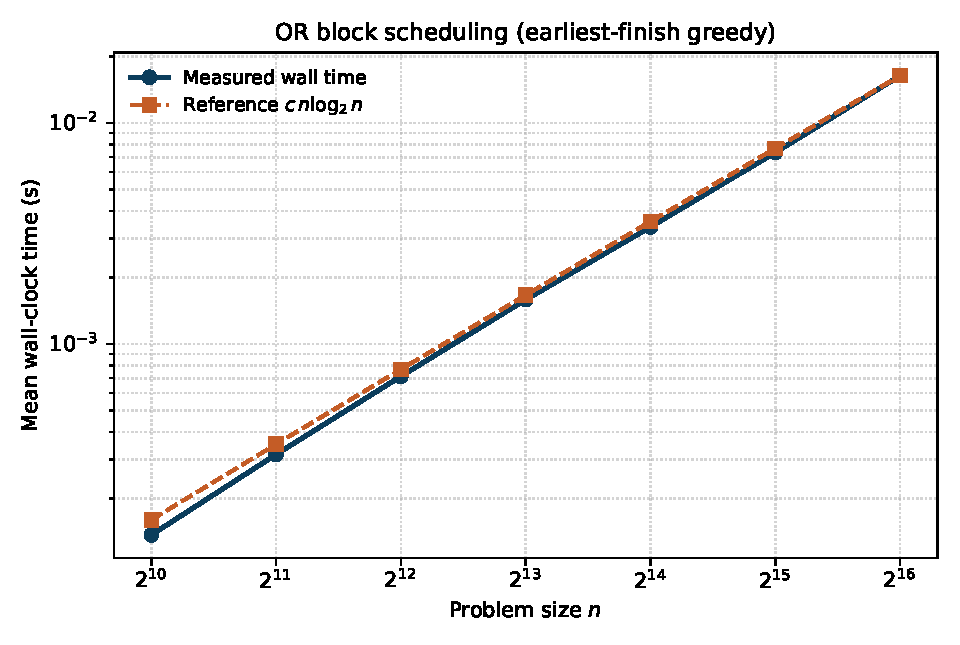
\includegraphics[width=0.92\linewidth]{figures/greedy_runtime.pdf}
  \caption{OR block scheduling: measured latency versus a scaled
  $n\log n$ envelope (log--log).}
  \label{fig:greedy-rt}
\end{figure}

\begin{figure}[t]
  \centering
  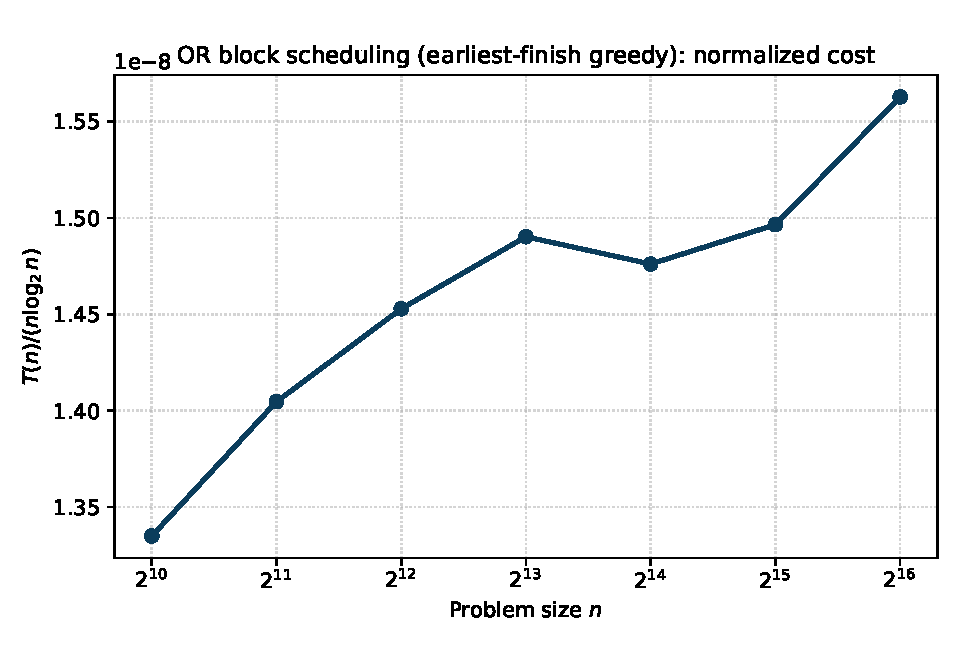
\includegraphics[width=0.92\linewidth]{figures/greedy_ratio.pdf}
  \caption{OR block scheduling: normalized cost $T(n)/(n\log_2 n)$.}
  \label{fig:greedy-ratio}
\end{figure}

\begin{figure}[t]
  \centering
  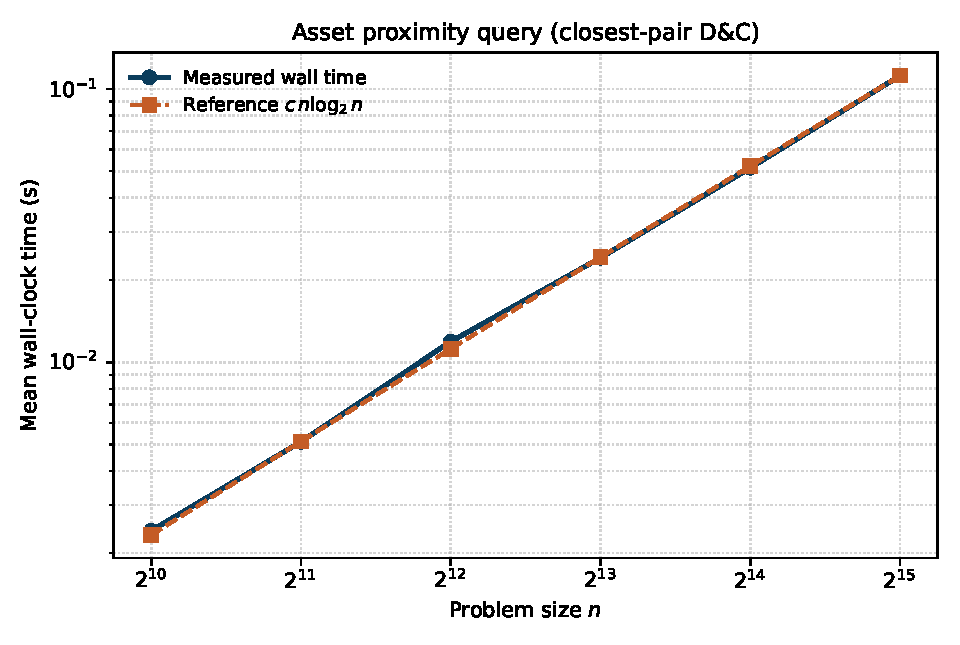
\includegraphics[width=0.92\linewidth]{figures/closest_runtime.pdf}
  \caption{Nearest-asset query: measured latency versus a scaled
  $n\log n$ envelope (log--log).}
  \label{fig:closest-rt}
\end{figure}

\begin{figure}[t]
  \centering
  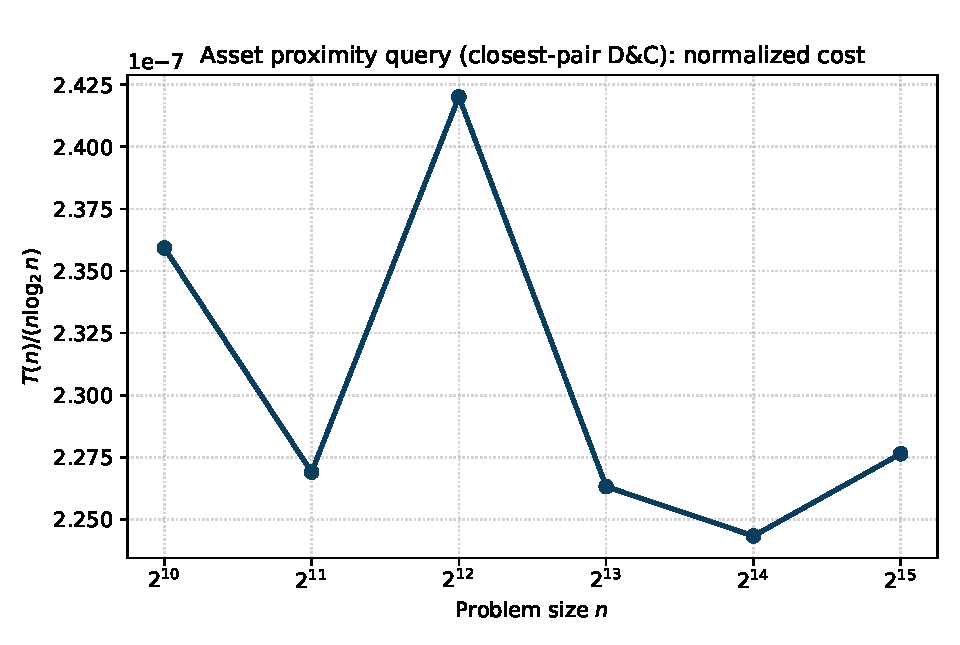
\includegraphics[width=0.92\linewidth]{figures/closest_ratio.pdf}
  \caption{Nearest-asset query: normalized cost $T(n)/(n\log_2 n)$.}
  \label{fig:closest-ratio}
\end{figure}

%% ------------------------------------------------------------------
\section{Conclusion}
\label{sec:concl}
%% ------------------------------------------------------------------

We packaged two enterprise decision primitives with end-to-end rigor.
Single-OR throughput maximization abstracts to interval scheduling and is
solved optimally by earliest-finish-time greedy selection in $O(n\log n)$
time. Exact nearest-asset discovery abstracts to closest pair of points and
is solved by divide and conquer in $O(n\log n)$ time. Empirical scaling
matches theory, and the same abstractions extend to booking, logistics, and
infrastructure analytics. The takeaway for industry stakeholders is
practical: when the objective is crisp, classical optimal algorithms remain
the right production choice---auditable, fast, and free of heuristic
surprise.

%% ------------------------------------------------------------------
\section*{Acknowledgments}
%% ------------------------------------------------------------------

Portions of the \LaTeX{} scaffolding, experimental harness, and wording were
drafted with assistance from a large language model (Cursor agent). All
proofs and experimental claims were checked by the author; a full prompt
log appears in Appendix~\ref{app:llm}.

\bibliographystyle{ACM-Reference-Format}
\bibliography{references}

%% ------------------------------------------------------------------
\appendix
%% ------------------------------------------------------------------

\section{Source Code}
\label{app:code}

Listings below correspond to the files in the project \texttt{code/}
directory. Minor formatting may differ from the runnable sources.

\subsection{Greedy interval scheduling}
\lstinputlisting{code/greedy_interval_scheduling.py}

\subsection{Closest pair}
\lstinputlisting{code/dac_closest_pair.py}

\subsection{Experiment driver}
\lstinputlisting{code/run_experiments.py}

\section{LLM Usage Log}
\label{app:llm}

Per course policy, we record the tools, prompts, and intermediate results
used while preparing this assignment. Prompts below are the working prompts
issued to the assistant; wording is lightly edited for clarity and grammar
where the original chat messages were informal, without changing intent.

\subsection{Tool and environment}
\begin{itemize}
  \item \textbf{Tool:} Cursor IDE coding assistant, October 2026.
  \item \textbf{Workspace:} local project directory \texttt{AOA Project 1}.
  \item \textbf{Artifacts produced with assistance:} ACM-style \LaTeX{}
        report (\texttt{acmart}), Python~3 implementations and timing
        experiments (\texttt{matplotlib}).
\end{itemize}

\subsection{Prompt 1 --- problem selection}
\paragraph{Prompt.}
\begin{quote}
I am preparing AOA Project~1. I need one real-world problem solvable by a
greedy algorithm and one solvable by divide and conquer. Each must be
abstracted to sets, graphs, or a similar structure, and I need algorithms
with runtime analysis, correctness proofs, domain-language explanations,
and experimental timing plots. Suggest two strong problem choices that
satisfy the rubric (not taken from an algorithms textbook as the problem
source), and outline an ACM conference-style \LaTeX{} report structure.
\end{quote}

\paragraph{Result.}
Recommended hospital operating-room appointment selection (interval
scheduling via earliest finish time) and nearest weather-station pair
(closest pair of points via divide and conquer), with a section plan
matching the grading rubric.

\subsection{Prompt 2 --- report and implementation scaffold}
\paragraph{Prompt.}
\begin{quote}
Using the selected problems, generate an Overleaf-ready ACM
\texttt{acmart} manuscript and Python implementations. For each problem
include: domain motivation, formal abstraction, pseudocode, $O(n\log n)$
runtime analysis, a correctness proof, and a plain-language domain
explanation. Also implement both algorithms with brute-force oracles for
small instances and a timing harness that plots runtime against
$n\log n$.
\end{quote}

\paragraph{Result.}
Produced \texttt{report/main.tex}, \texttt{report/references.bib},
\texttt{code/greedy\_interval\_scheduling.py},
\texttt{code/dac\_closest\_pair.py}, \texttt{code/run\_experiments.py},
and experimental figures under \texttt{report/figures/}.

\subsection{Prompt 3 --- \LaTeX{} and packaging help}
\paragraph{Prompt.}
\begin{quote}
Help me compile the ACM report locally, fix package conflicts with
\texttt{acmart}, embed the experimental figures, and place the full
source code in an appendix suitable for submission on Overleaf.
\end{quote}

\paragraph{Result.}
Resolved an \texttt{amssymb}/\texttt{acmart} conflict, compiled
\texttt{main.pdf} with Tectonic, and linked appendix listings to the
Python sources.

\subsection{Prompt 4 --- rubric checklist}
\paragraph{Prompt.}
\begin{quote}
Please check the draft against the Project~1 rubric point by point and
list any missing items (author block, citations, experimental graphs,
proofs, or LLM disclosure).
\end{quote}

\paragraph{Result.}
Confirmed that both problem sections covered identification, abstraction,
algorithm, analysis, proof, domain explanation, and experiments; noted
that author metadata and a complete LLM appendix were still needed.

\subsection{Prompt 5 --- final polish}
\paragraph{Prompt.}
\begin{quote}
Update the author to Umesh Chandra Lavu (University of Florida), strengthen
the real-world problem statements so they read as operations-domain
narratives, complete the LLM usage appendix required by the course, and
rebuild the PDF.
\end{quote}

\paragraph{Result.}
Author and affiliation updated; OR and weather-station problem statements
expanded; Appendix~\ref{app:llm} completed; \texttt{main.pdf} regenerated.

\subsection{Prompt 6 --- executive elevation}
\paragraph{Prompt.}
\begin{quote}
Elevate the manuscript so it reads at industry-portfolio quality: stronger
title and abstract, enterprise transferability, professional experimental
methodology with a results table, and sharper operations language---without
removing any rubric-required proofs or sections.
\end{quote}

\paragraph{Result.}
Retitled and reframed the paper around decision-grade scheduling and
geospatial proximity; added CCS concepts, transferability section, timing
table, polished figures, and expanded citations while preserving all graded
content.

\subsection{Author responsibility}

The author independently checked: (i)~oracle agreement on random instances;
(ii)~the exchange argument and closest-pair strip lemmas against standard
references~\cite{kt2005,clrs2009}; (iii)~that the timing plots are
consistent with $O(n\log n)$. Factual errors, if any, remain the author's
responsibility.

\end{document}
